
\section{Trapped Ion Quantum Computing \cite{bruzewiczTrappedionQuantumComputing2019}} \label{sec:Trapped}
In this section we provide an introduction to the implementation details of trapped ion quantum computers (**once done possibly elaborate what exactly we covered).
The qubits in a trapped ion system are represented by individual trapped ions.
As would have been seen in a quantum mechanics class, electrons bound in atoms can occupy a certain number of possible quantum states, here 2 of these level are chosen and used as the \kz and \ko states.
Though it isn't quite as simple as that, for quantum computing we must have a way of entangling these 2 states.
To achieve that, the qubit ions are trapped in the same trap (explained later on) and their motion within it is coupled as a quantum system, through which entanglement is achieved.
The rest of the required features for quantum computing including state preparation, readout and quantum gates are all achieved through tuned lasers and or the mentioned entanglement.

\subsection{Ion Trapping and the Paul Trap}
Ion trapping is an extensive field of expertise used for many purposes across physics and other sciences, it is an essential component of many devices and experiments that try to manipulate individual particles, molecules or so on.
For a brief sketch of what this involves, these experiments must be done in vacuum (otherwise there would be too many other atoms around) and rely on complex electric and magnetic fields to manipulate the motion of charged atoms.
For quantum computing we are interested in trapping individual ions in a stable way, and while we want to trap multiple of them (currently about 5-100 has been achieved \cite{paganoCryogenicTrappedionSystem2018}) it is important that we can tell them apart (as opposed to trapping them in bunches as is often done).

There are currently 2 dominant, suitable classes of ion traps, Penning traps which uses a combination of magnetic and electric fields, and Paul traps (also known as Quadrupole or Radio-Frequency-Quadrupole ion traps) which uses time varying electric fields.
Penning traps are able to hold larger amounts of ions and more stably (300 ion crystals have been achieved \cite{bohnetQuantumSpinDynamics2016}), however the motion of the ions themselves is much more complicated and leads to qubit manipulation being harder to perform.
Because of that Paul traps are more commonly used for quantum computers and due to the scope of this report we will focus on them.

\subsubsection{Simple Paul Trap}
Paul trap designs use time varying fields as it is not possible to confine an ion in 3D space with only static fields.
The simplest Paul trap design is composed of 4 conducting rods run in parallel to create a quadrupole electric field in the middle (\cref{fig:TIQC_RFQ_Flour} shows a demonstrative model).
Then have each of the diagonally opposite rods connected at the same voltage and have these 2 voltages be some periodic function (usually a sine or a square wave at approximately radio frequencies, hence the name) in antiphase, so that if at some time one pair is set to positive voltage, the other should be at negative voltage.
This results in a net effect of trapping a charged particle (within some range of mass to charge ratios of the ions, the setup can be used as a mass filter) along the axis of the quadrupole, why exactly this is so is well explained in (**add a source here).
Finally, for trapping along the last axis a static electric field is used, this can be achieved by for example 2 more rod segments along the quadrupole axis at either end of the whole setup, both at some positive voltage, resulting in a potential well along the axis.

\begin{figure}[H]
    \centering
    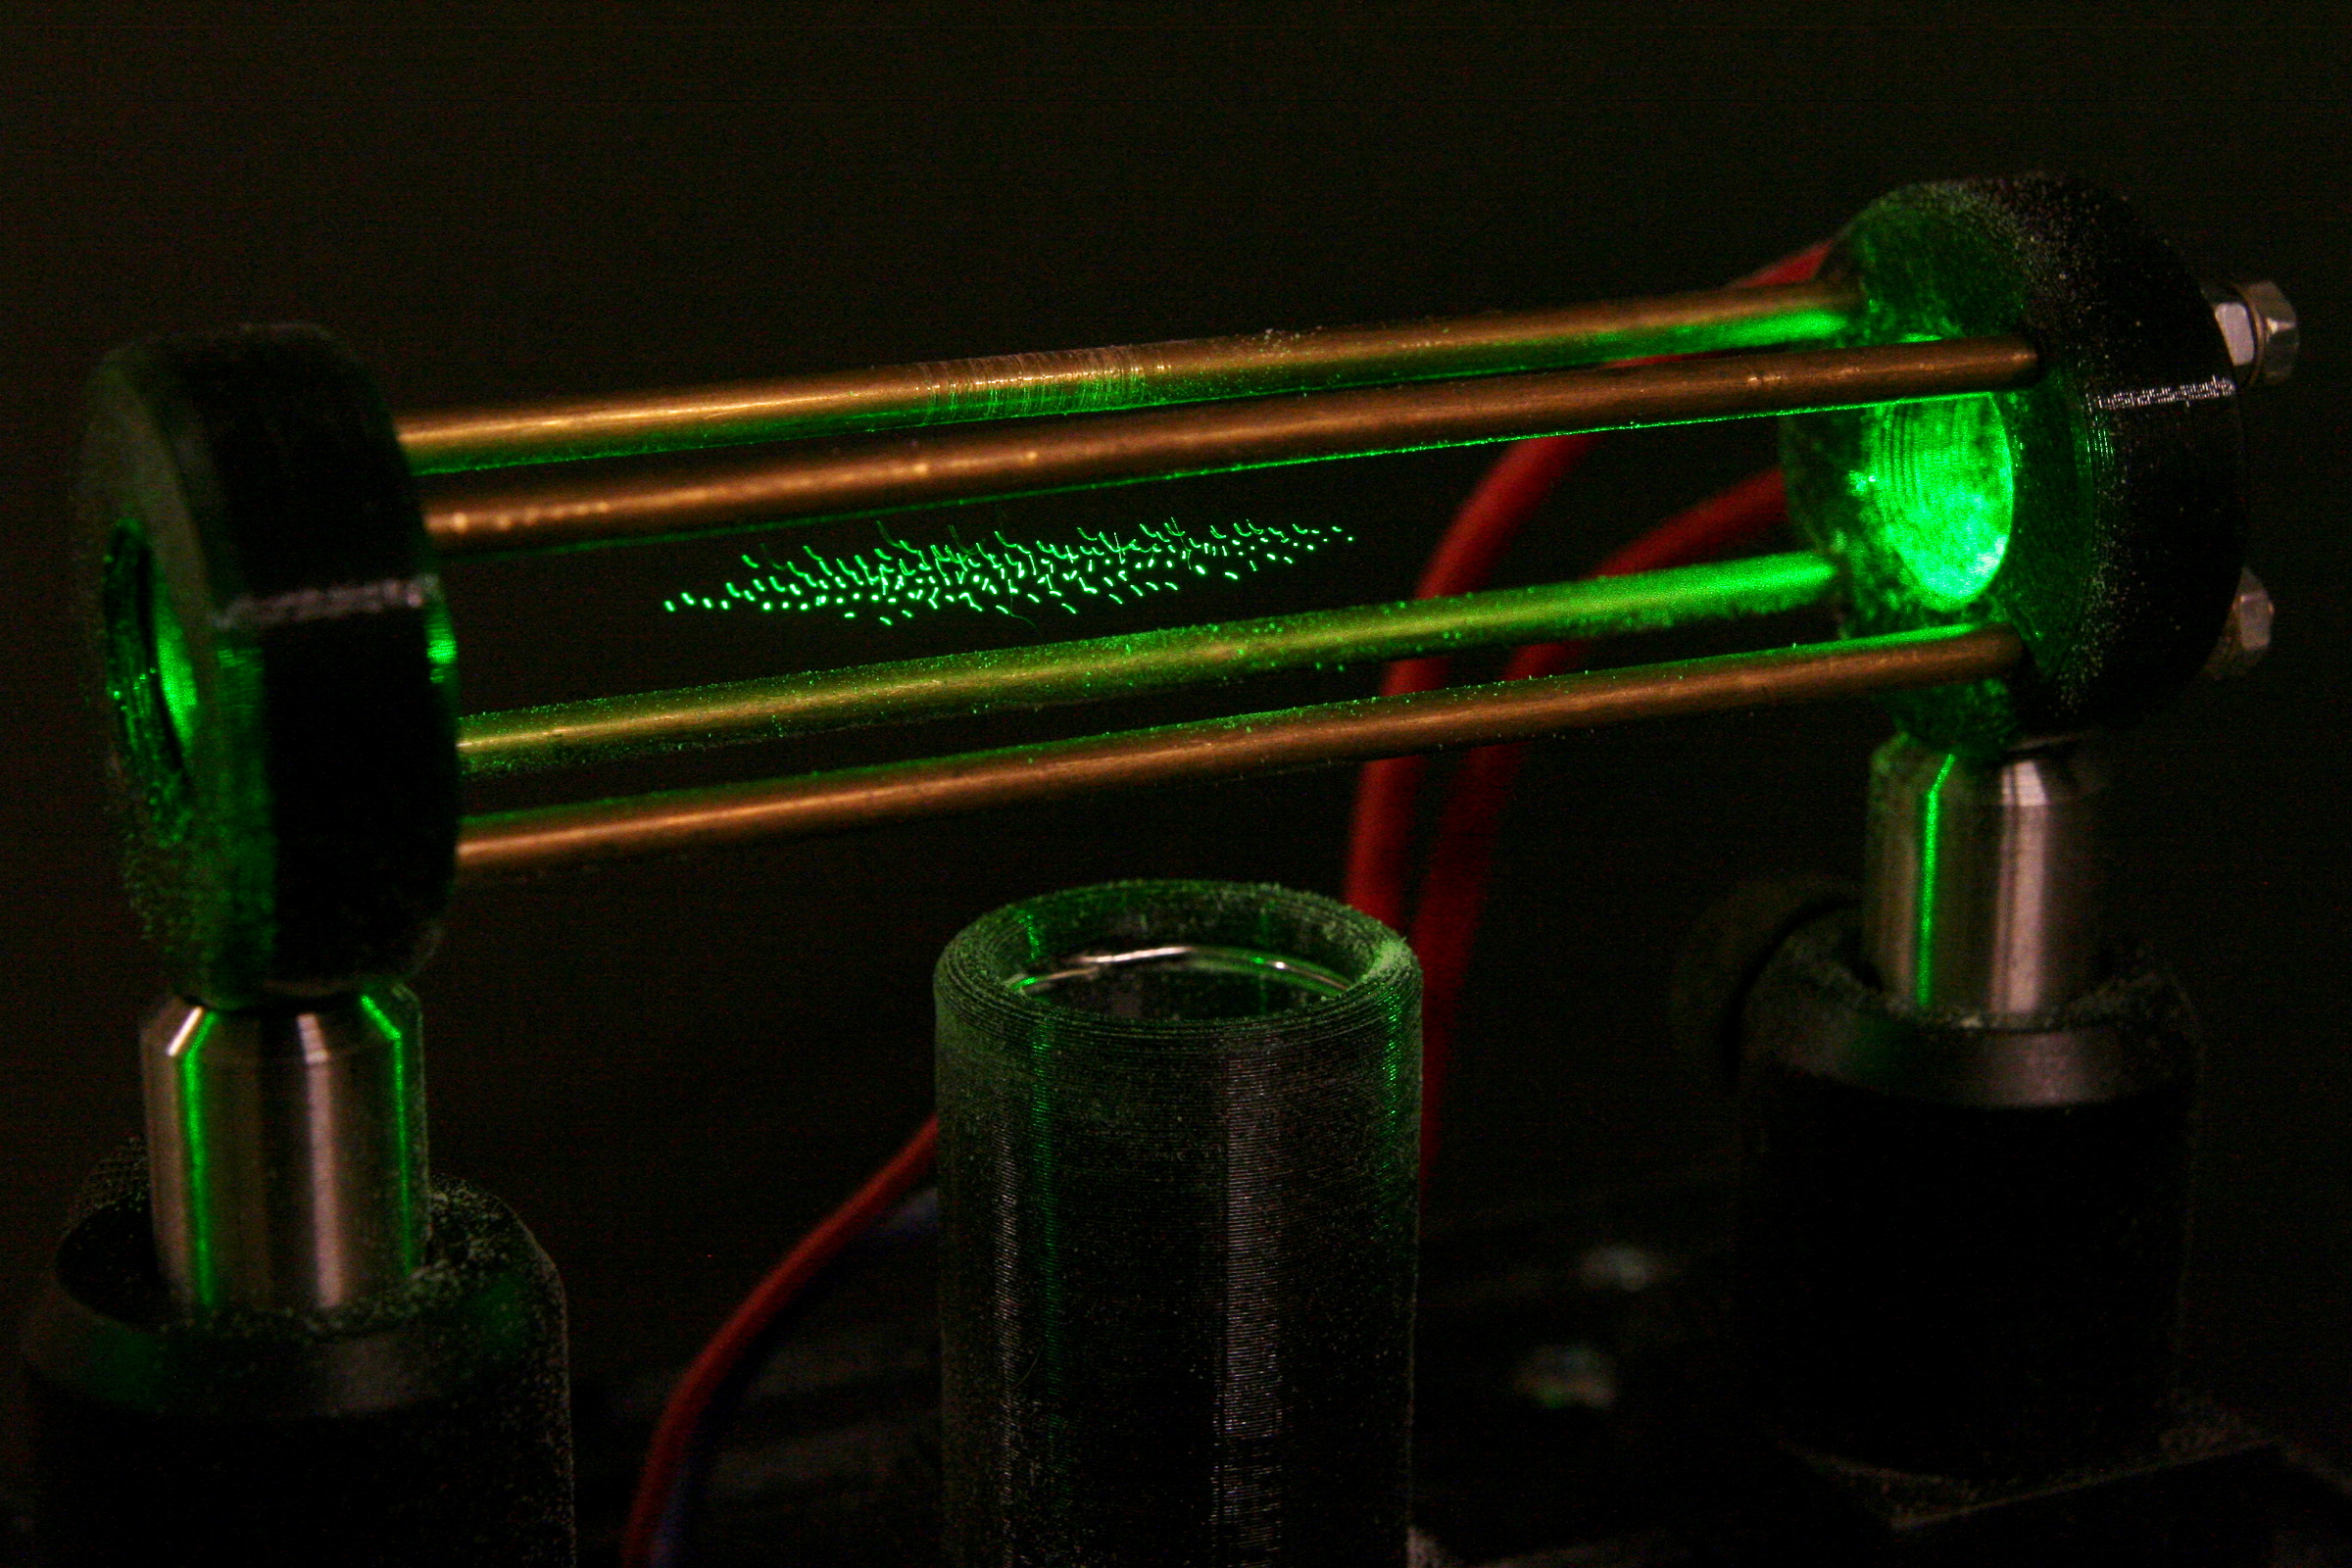
\includegraphics[width=0.9\textwidth]{images/TIQC_RFQ_Flour.jpg}
    \caption{Charged flour grains trapped in a simple Paul trap, the mentioned 4 parallel rods are visible and the electrodes creating the potential well are in the end caps.(**cite Pavelka, found on wikipedia)}\label{fig:TIQC_RFQ_Flour}
\end{figure}

\subsubsection{Notes on Other Paul Trap Designs}
The aforementioned simple Paul trap is in fact a linear Paul trap, in this type of Paul traps the ion's motion is confined in 2 dimensions by an RF quadrupole and the last is taken care of using a linear static potential, this is the type of trap on which we will focus.
There are also point Paul traps, which utilise oscillating RF fields for trapping in all 3 dimensions, these are also used for quantum computing, however when multiple ions are trapped together (which is necessary for entanglement) their motion is significantly more complex.

However there is still a plethora of different designs being explored for further progress, most interestingly there are "surface" Paul traps.
These are usually microfabricated plates with a layout of electrodes on their surface which when driven by the correct voltages give rise to a trapping field above their surface.
These designs offer great advantages for quantum computing, as not only are they cheaper and quicker to manufacture, but can be produced with a much higher precision than manually assembled devices.
They also have the benefit of the trapped ions being much more accessible for manipulation through lasers.
Recently chips with integrated photonics have been developed too, these are surface Paul traps with optical channels running through them with openings in the surface aimed at the ion see \cref{fig:TIQC_MIT} for diagrams of one developed at MIT \cite{niffeneggerIntegratedMultiwavelengthControl2020}.
This further reduces the need for precision assembly and calibration, however complications arise with generating and maintaining entangled states if each ion is stored separately in these modules \cite{bruzewiczTrappedionQuantumComputing2019}.


\begin{figure}[H]
    \centering
    \begin{subfigure}[b]{0.45\textwidth}
        \centering
        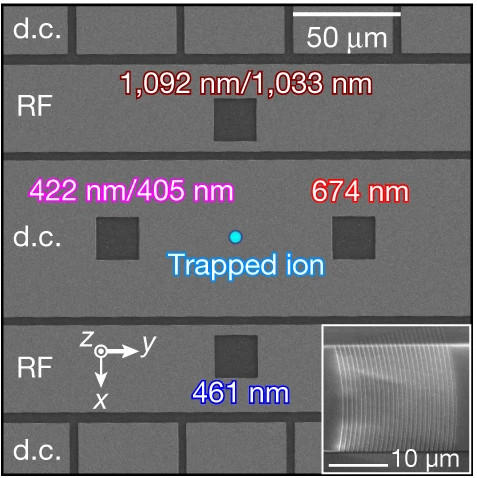
\includegraphics[width=0.9\textwidth]{images/TIQC_MIT_1.jpg}
        \subcaption{Layout of the surface Paul trap}
    \end{subfigure}
    \hfill
    \begin{subfigure}[b]{0.45\textwidth}
        \centering
        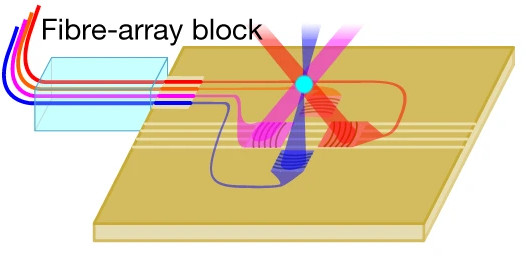
\includegraphics[width=0.9\textwidth]{images/TIQC_MIT_2.jpg}
        \subcaption{Diagram showing the photon beams}
    \end{subfigure}
    \caption{Surface Paul trap with integrated photonics for quantum computing developed at MIT in 2020.}\label{fig:TIQC_MIT}
\end{figure}

\subsection{The ions and types of qubits}
As the trapping was briefly covered, the next logical step is to focus on the ion itself.
First question is what element should be use and some of the main requirements are that it is radioactively stable, can be easily produced, can singly ionized and finally that it has 2 suitable states to use as \kz and \ko.
For this, the valence electron (also the one that is "free" due to ionization) is the important part, the energy levels available to it are used as our needed states.

For a quick summary of atomic structure, an electron is bound to the nucleus by the Coulomb interaction, if this is considered only and the quantum problem is solved, we get the gross structure, giving rise to different energy levels with different quantum numbers n.
The next step is to consider the interaction between the electrons spin and angular momentum, and also certain relativistic corrections.
This gives rise to the fine structure which are the usual orbitals described by the quantum numbers: the same n, l usually given letters s, p, d and so on, and the total spin j.
Next, there is another correction which comes from the interaction between the electron's spin and the total spin of the nucleus (if non-zero).
This gives rise to more splitting and the resulting energy levels are called the hyperfine structure.
Finally, in very vague terms, if an atom is in a magnetic field there is again more splitting, this is called the Zeeman effect.
Details on all of this can be found in \cite{woodgateELEMENTARYATOMICSTRUCTURE1970} and a diagram of the typical fine structure of the ions used for trapped ion QC along with some of the zeeman and hyperfine splittings are shown in \cref{fig:TIQC_levels}.

Coming back to quantum computing there are many options for our states and they can usually be classified as one of following types.

\begin{figure}[H]
    \centering
    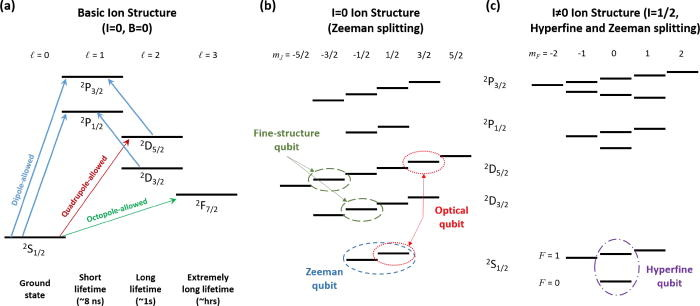
\includegraphics[width=0.9\textwidth]{images/TIQC_levels.jpeg}
    \caption{Fine structure and Zeeman and hyperfine splittings of typical atoms used for quantum computing. Some of the possible choices for the sates are also shown.}\label{fig:TIQC_levels}
\end{figure}

\subsubsection{Zeeman qubits}
Zeeman qubits are qubits where the 2 states are in the same hyperfine and fine structure orbital, but result from the Zeeman effect.
They offer near infinite lifetimes and most operations can be done relatively simply, but their main drawback is that these states are very sensitive to magnetic field fluctuations (they arise from external magnetic fields after all).
This limits their coherence times, however coherence times of 300 ms have been achieved \cite{rusterLonglivedZeemanTrappedion2016}

\subsubsection{Hyperfine qubits}
With these the 2 states are hyperfine split levels from the ground state.
Among their advantages are also an near infinite lifetime and possibly and an easier read out than Zeeman qubits along with a relative insensitivity to magnetic field fluctuations.
The main drawback to them is the more complicated structure of the energy levels, thus requiring greater precision in laser frequencies \cite{bruzewiczTrappedionQuantumComputing2019}.

\subsubsection{Optical qubits}
In some ions it is possible to use an S and a D level as our states, this has the benefit of very simple level structure.
However these D states are only metastable, of lifetimes on the order of seconds \cite{ozeriTrappedionQubitTool2011}.
Furthermore, the more precise the laser frequencies are the longer the achieved lifetimes are, however as the energy gap is relatively large for these states, the required lasers for manipulation need to have frequencies of visible to infrared light (hence the name).
As suitable laser precisions are very hard to attain optical qubits tend to be less popular, however their popularity is growing with advances in laser sources \cite{bruzewiczTrappedionQuantumComputing2019}.
% However as the energy gap gets bigger so does the required lasers wavelength and for optical qubits the frequencies are of visible to infrared light (hence the name) and achieving the required frequency precision is a very difficult task.

\subsubsection{Fine structure qubits}
This type of qubit uses 2 of the D levels mentioned in the last section.
The obvious downside is then their short lifetimes, however as the energy gap between these levels is much smaller, higher frequency precision can be more easily attained in the required lasers.
As a downside comes a more complicated level structure, for example the readout has to be done by first transferring one of the possible states to another one before reading out.


Overall there is not a clear winner and which choice is made depends on the particulars of the given company or research team, depending on their expertise and the equipment available to them.

% some of the main requirements for a suitable isotope is that it is radioactively stable, can be produced, is singly ionizable and most importantly that the valence electron has suitable stable available quantum mechanical states to occupy, to use for \kz and \ko.
% Group 2 elements or similar (namely group 12 elements and Yb \cite{ozeriTrappedionQubitTool2011}) are typically used, as they have a full shell except a single valence electron.
% However for many of them, there are multiple suitable electron states available for use, based on which are used the qubits would be classified as Zeeman, Hyperfine, Optical or Fine-structure.
% To summarize what these are, in either case we start with the typical electron orbitals around an atom


\subsection{Qubit (ion) manipulation, the lasers for state prep, readout and so on, and entanglement!}

TODO
\begin{itemize}
    \item Mention DiVincezo in above, essentially what was now described is how the \kz and \ko states are stored
    \item motional states! and entanglement through them, can get long
    \item actual manipulation - ideally structure along DiVincezo
\end{itemize}

